%%==================================================================%%
%% Author : Tejedo Gonz�lez, Daniel                                 %%
%%          S�nchez Barreiro, Pablo                                 %%
%% Version: 1.0, 25/11/2012                                         %%
%% Version: 2.0, 06/02/2013                                         %%
%%                                                                  %%
%% Memoria del Proyecto Fin de Carrera                              %%
%% Sintaxis abstracta, archivo ra�z                                 %%
%%==================================================================%%

\chapterheader{Desarrollo de la Sintaxis Abstracta}{Desarrollo de la Sintaxis Abstracta}
\label{chap:metamodelo}

El presente cap�tulo describe el proceso de desarrollo de nuestra primera tarea de acuerdo al proceso de desarrollo dirigido por modelos de nuestro lenguaje. Dicha tarea es el desarrollo de un metamodelo o sintaxis abstracta para nuestro lenguaje.

\chaptertoc

\section{Introducci�n}
\label{sec:meta:requisitos}
%%==================================================================%%
%% Author : Abascal Fern�ndez, Patricia                             %%
%% Author : S�nchez Barreiro, Pablo                                 %%
%% Version: 1.2, 24/06/2013                                         %%
%%                                                                  %%
%% Memoria del Proyecto Fin de Carrera                              %%
%% Application Engineering/Introduccion                             %%
%%==================================================================%%

Este cap�tulo describe el proceso de desarrollo de los generadores de c�digo para la segunda fase del desarrollo de una l�nea de productos software (ver Figura~\ref{back:fig:domainAplicEng}), el proceso de \emph{Ingenier�a de Aplicaciones}. El objetivo de esta fase, tal como comentamos, es obtener productos concretos y funcionales a partir de la composici�n, configuraci�n y personalizaci�n de los elementos creados en la fase de \emph{Ingenier�a del Dominio}.

Para ello, de acuerdo con la metodolog�a Te.Net (ver Secci�n~\ref{sec:intr:tenet}), el primer paso es crear una selecci�n de aquellas caracter�sticas que se desea incluir en el producto, de acuerdo a las necesidades particulares de cada cliente. C�mo se crea dicha selecci�n de caracter�sticas est� fuera del �mbito de este proyecto. Referimos al lector interesado al Proyecto Fin de Carrera de D. Daniel Tejedo, antiguo alumno de esta Facultad~\citep{daniel:2013}.

Una vez obtenida una selecci�n de caracter�sticas v�lida, utilizando dicha selecci�n, se configura la arquitectura de referencia creada en la fase de \emph{Ingenier�a del Dominio} para crear un modelo arquitect�nico concreto, adaptado a las necesidades del cliente, del producto que queremos construir.  Dicho modelo arquitect�nico se obtiene de forma autom�tica mediante la utilizaci�n del lenguaje \emph{VML}~\citep{loughran:2008,sanchez:2008}, de acuerdo con la metodolog�a Te.Net (ver Secci�n~\ref{sec:intr:tenet}). Una descripci�n detallada del lenguaje VML tambi�n est� fuera del �mbito de este proyecto, y referimos al lector interesado al trabajo de~\cite{daniel:2013}.

Este modelo arquitect�nico de un product concreto es el que sirve de entrada al generador de c�digo que queremos desarrollar. Utilizando dicho modelo como entrada, el generador de c�digo debe producir todo el c�digo necesario para componer las clases parciales creadas a nivel de \emph{Ingenier�a del Dominio} que correspondan. Para ello debe generar las clases parciales encargadas de llevar a cabo tal composici�n, las versiones limpias de los m�todos requeridos, y las delegaciones a las versiones sucias adecuadas.

Para ello, el primer paso era dise�ar un algoritmo que permitiese calcular estos tres elementos: (1) clases parciales requeridas; (2) versiones limpias necesarias; y, (3) delegaciones adecuadas. A continuaci�n, deb�amos implementar este algoritmo utilizando plantillas de generaci�n de c�digo, por lo que deb�amos, igual que en cap�tulo anterior, prestar especial atenci�n a su secuenciaci�n.

Por �ltimo, deb�amos dise�ar y realizar las pruebas que permitiesen comprobar el correcto funcionamiento del generador de c�digo. Tras estas pruebas, se daba por concluido el proceso de desarrollo de los generadores de c�digo, y procedimos a su despliegue.

Para explicar este proceso de desarrollo, este Cap�tulo se estructura como sigue: La Secci�n~\ref{application:sec:alg} describe la estructura de los modelos de entrada que nuestro generador de c�digo debe procesar. La Secci�n~\ref{application:sec:alg} describe el dise�o del algoritmo encargado de calcular los elementos a componer, de acuerdo al modelo de entrada proporcionado. La Secci�n~\ref{application:sec:transf} explica c�mo se han secuenciado las plantillas de generaci�n de c�digo para poder implementar dicho algoritmo. La Secci�n~\ref{application:sec:pruebas} describe el proceso de dise�o y ejecuci�n de las pruebas para el generador de c�digo implementado. Por �ltimo, la Secci�n~\ref{application:sec:despliegue} detalla las acciones realizadas durante la fase de despliegue de la aplicaci�n.








\section{Captura de requisitos}
\label{sec:meta:requisitos}
%%==================================================================%%
%% Author : Tejedo Gonz�lez, Daniel                                 %%
%%          S�nchez Barreiro, Pablo                                 %%
%% Version: 1.0, 27/11/2012                                         %%                   
%%                                                                  %%
%% Memoria del Proyecto Fin de Carrera                              %%
%% Gram�tica,  requisitos                                           %%
%%==================================================================%%

La captura de requisitos de la gram�tica pasa por informarse sobre qu� tipo de sintaxis textual queremos que tengan nuestras operaciones, lo cual en este caso ya estaba especificado previamente por documentos creados en iteraciones previas del proyecto Hydra. Lo m�s l�gico e inmediato era mantenerse fiel a esa sintaxis, seg�n la cual las operaciones deber�an ser expresadas textualmente tal como sigue: \\

Suma: operando1 + operando2

Resta: operando1 - operando2

Multiplicaci�n: operando1 * operando2

Divisi�n: operando1 / operando2

And: operando1 and operando2

Or: operando1 or operando2

Xor: operando1 xor operando2

Implica: operando1 implies operando2

Mayor que: operando1 > operando2

Menor que: operando1 < operando2

Igual que: operando1 == operando2

Mayor o igual que: operando1 >= operando2

Menor o igual que: operando1 <= operando2

Distinto que: operando1 != operando2

Contexto: operando1 [ operando2 ]

Para todo: all operando1 [ operando2 ]

Existe: any operando1 [ operando2 ] \\

Otros aspectos concernientes a la gram�tica que ha habido que tener en cuenta dentro de la fase de captura de requisitos son los siguientes:\\

- Ha de permitirse la posibilidad de especificar prioridad en las operaciones, es decir, de poder delimitar las operaciones con par�ntesis que denoten el orden de realizaci�n de las mismas.

- Todas las representaciones textuales de nuestro lenguaje han de empezar con una l�nea de carga del modelo de caracter�sticas al que han de aplicarse las restricciones. La sintaxis de este aspecto ser� "import operando", donde operando es la direcci�n del fichero hydra del modelo dentro del disco duro del sistema.

- Todas las restricciones definidas han de separarse entre ellas mediante el car�cter '' ; ''.\\

Por supuesto, adem�s de los requisitos aqu� expuestos tambi�n habr� que tener en cuenta todo lo comentado en el apartado de requisitos del cap�tulo anterior, ya que tambi�n influir�n a la hora de tomar decisiones de dise�o en la gram�tica.


\section{Creaci�n del metamodelo}
\label{sec:meta:creacion}
%%==================================================================%%
%% Author : Tejedo Gonz�lez, Daniel                                 %%
%%          S�nchez Barreiro, Pablo                                 %%
%% Version: 1.0, 25/11/2012                                         %%                   
%%                                                                  %%
%% Memoria del Proyecto Fin de Carrera                              %%
%% Sintaxis abstracta, creacion metamodelo                          %%
%%==================================================================%%

Una vez hemos conocidos cu�les son los requisitos que deb�a satisfacer nuestro lenguaje, procedimos a construir un metamodelo en Ecore que cumpla tales requisitos. Dicho metamodelo se muestra en la Figura~\ref{figmetameta}.

%%==================================================================%%
%% NOTA(Pablo): Intenta meter esta figura de forma apaisada         %%
%%              Intenta que la figura se vea menos borrosa.         %%
%%              Intenta que la figura tenga menos cruces de linea   %% 
%%              �Es una captura de pantalla?                        %% 
%%==================================================================%%

\begin{figure}[!tb]
    \centerline{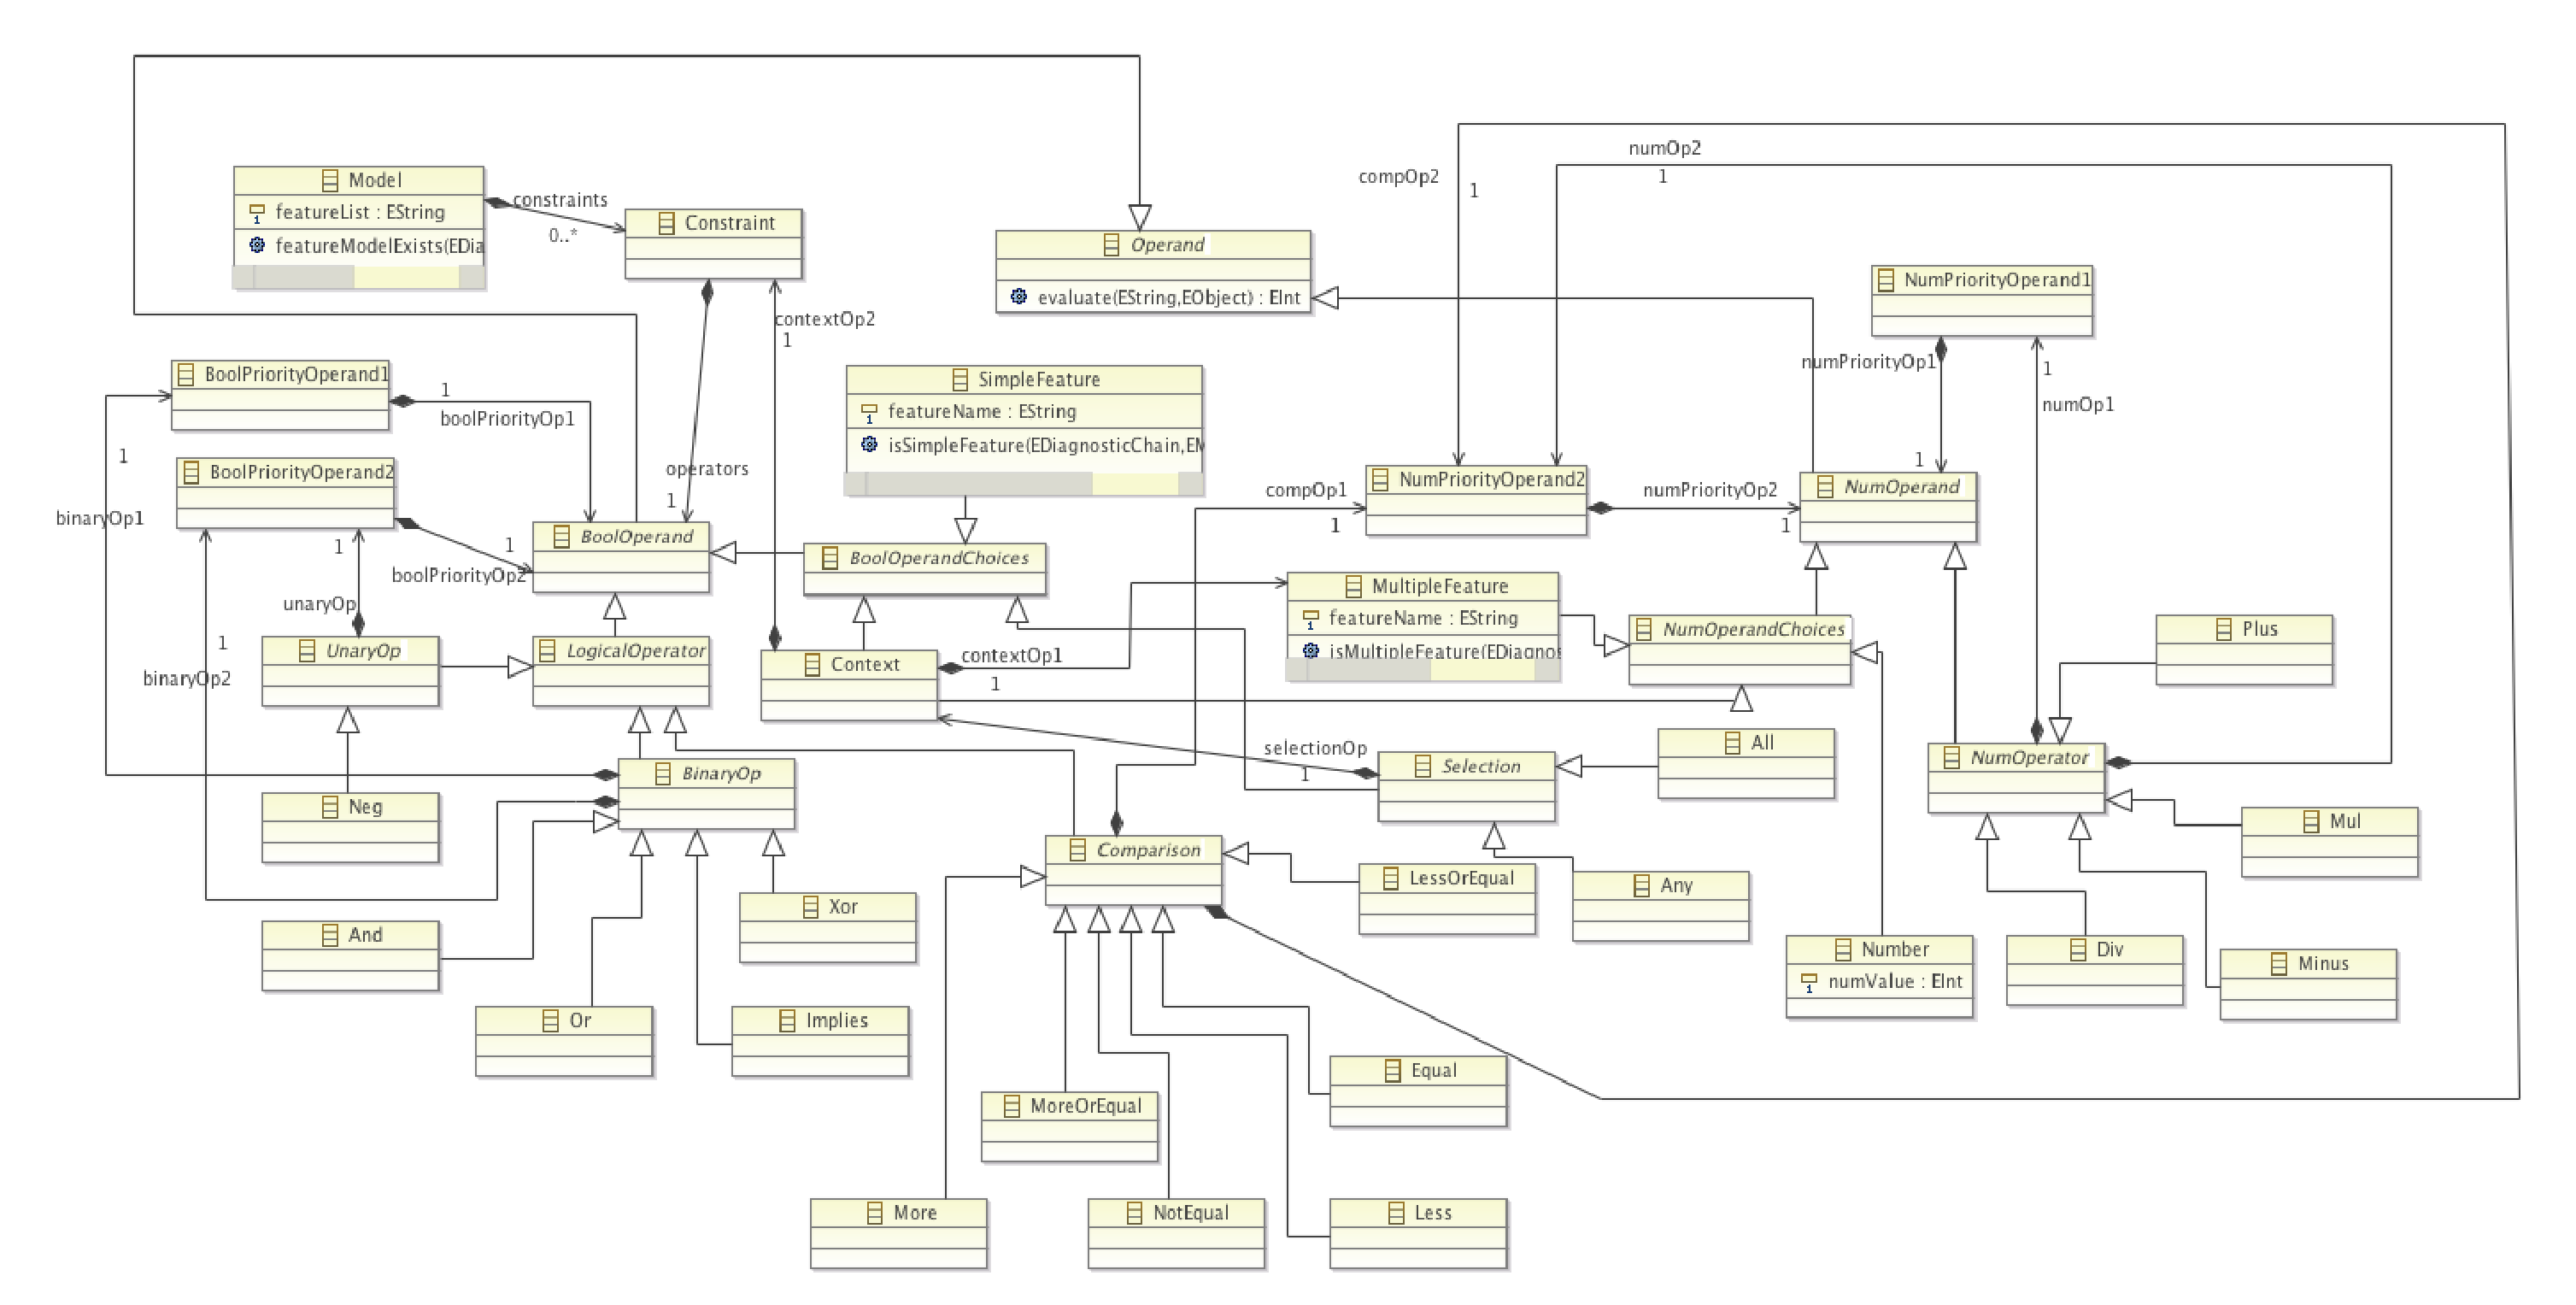
\includegraphics[scale=0.38, angle=90]{metamodelo/metamodelo.eps}}
    \caption{Metamodelo para el lenguaje HCL}
    \label{figmetameta}
\end{figure}

La clase \emph{Model} es la que sirve de punto de entrada y contender para el resto de las clases de nuestro metamodelo. 

C�mo se ha comentado anteriormente, debemos vincular un conjunto de restricciones con el �rbol de caracter�sticas al cual deben aplicarse. Dicho �rbol de caracter�sticas debe haber sido previamente creado usando la herramienta \emph{Hydra}, de acuerdo con los objetivos generales del proyecto. Eso reduce mucho el n�mero de factores de los que hay preocuparse, vi�ndose reducidos en este punto a tener que almacenar �nicamente la localizaci�n del fichero que contiene dicho �rbol de caracter�stica, con objeto de poder cargarlo cuando se necesite. La ruta de dicho fichero se almacena en el atributo \emph{featureList} de la clase \emph{Model}.

Un modelo de restricciones permite especificar un n�mero indeterminado de restricciones, representadas por la clase \emph{Constraint}. Por tanto, la clase \emph{Model} contendr� 0 o m�s restricciones (en principio se permiten definir ficheros sin restricciones, que se entiende se refinar�n postriormente). 

Una restricci�n es una expresi�n booleana que se eval�a a vedadero o falso, y que contendr� un operador booleano, representando por la clase \emph{BoolOperand}, y varios operadores, representados por diversas clases. 

Un operador booleano puede ser tanto una \emph{SimpleFeature}, es decir, una caracter�stica no clonable, como una operaci�n cuya evaluaci�n de como resultado un valor booleano. Estas operaciones pueden ser l�gicas (\emph{and}, \emph{or}, \emph{implies}, \emph{xor} y \emph{not}), de comparaci�n ($<$, $<=$, $>$, $>=$, =, !=), de selecci�n (\emph{all} y \emph{any}) o de contexto.

Por otro lado, una restricci�n tambi�n puede contener operadores num�ricos. Un operador num�rico puede ser una \emph{MultipleFeature}, es decir, una caracter�stica clonable, un n�mero, o una operaci�n cuya evaluaci�n de como resultado un valor num�rico. Estas operaciones son artim�ticas, es decir, $+$, $-$, $*$ y $/$. El operador m�s prioritario de una restricci�n siempre ha de ser booleano, pues en �ltima instancia esta tiene que poder ser evaluada a verdadero o falso.

Las operaciones l�gicas y num�ricas descritas est�n representadas en el metamodelo mediante las metaclases que llevan su nombre. Es decir, \emph{LessOrEqual} es la operaci�n $<=$, \emph{Plus} es la operaci�n $+$, y as� sucesivamente. Se puede apreciar que estas metaclases son las hojas de una estructura de herencias. Esta estructura permite no solo facilitar la comprensi�n del metamodelo, sino tambi�n servir de apoyo a \emph{EMFText} en el momento de construir la posterior gram�tica. 

Como ejemplo, vamos a seguir esta estructura a trav�s de una de las operaciones, \emph{Implies}. Esta metaclase hereda de \emph{BinaryOp}, que es la metaclase que representa las operaciones l�gicas con dos operandos. \emph{BinaryOp} a su vez hereda de \emph{LogicalOperator}, que representa las operaciones l�gicas. Por �ltimo, \emph{LogicalOperator} hereda de \emph{BoolOperand}, que representa los operadores booleanos. Un an�lisis an�logo se podr�a realizar con cualquiera de las operaciones implementadas.

Cabe tambi�n mencionar algunas metaclases como \emph{BoolPriorityOperand1} que parecen ajenas a esta estructura y cuya presencia puede resultar dudosa. Su inclusi�n se justifica por razones de funcionamiento de la herramienta \emph{EMFText}, que requiere un tratamiento especial a la hora de implementar prioridad entre las operaciones.

Los atributos de las metaclases sirven para almacenar informaci�n importante para el lenguaje, que posteriormente podr�a ser utilizada a nivel de validaci�n o ejecuci�n. De estos atributos ya se ha mencionado la utilidad de \emph{featureList}, dentro de la clase \emph{Model}. Adem�s de este, el atributo \emph{featureName} de las clases \emph{SimpleFeature} y \emph{MultipleFeature} sirve para almacenar el nombre de la caracter�stica a la que hagan alusi�n. Por �ltimo, el atributo \emph{numValue} de la clase \emph{Number} sirve para guardar el valor literal num�rico que haya sido introducido.

%\todo{sigue t� describiendo el metamodel o en este estilo, describiendo su estructura sin entrar en detalles ni ponerte demasiado barroco. Describes lo que hay, no el proceso de c�mo lo hiciste ni si te cost� m�s o menos, o te pareci� f�cil o dificil. No describas las asociaciones entre metaclases, eso es demasiado detalle}.

%%========================================================================================%%
%% NOTA(Pablo): Todo lo de abajo quedar� redundante con el nuevo texto, as� que mejor     %%
%%              eliminarlo                                                                %% 
%%========================================================================================%%

%%========================================================================================%%
%% INICIO DE PARTE POSIBLEMENTE REDUNDANTE                                                %%
%%========================================================================================%%

%El primer paso es definir toda la estructura necesaria para la implementaci�n de las operaciones, haciendo que cada una de ellas est� representada en nuestro metamodelo mediante una clase, pero sin preocuparnos todav�a por las relaciones entre ellas. La clase ra�z de toda esta estructura es Operand. Es una clase abstracta, es decir, en los modelos que luego instanciemos de este metamodelo no podr� haber ninguna instancia de Operand, s�lo de los hijos no abstractos que tenga. A medida que vayamos definiendo clases hijas  de Operand estaremos especificando cada vez con m�s exactitud a qu� tipo de operaci�n estamos haciendo referencia.
%
%En el segundo nivel de la estructura de implementaci�n de las operaciones hacemos una ramificaci�n seg�n el tipo del valor de retorno o de evaluaci�n de las posibilidades. Es decir, a la clase Operand le a�adiremos dos hijos: BoolOperand para operaciones que se eval�an a booleano y NumOperand para operaciones que se eval�an a num�rico. Estas clases tambi�n ser�n abstractas.
%
%El proceso de divisi�n a partir de aqu� es m�s o menos an�logo para todas las operaciones, as� que vamos a centrarnos �nicamente en la rama que da lugar a las operaciones binarias l�gicas, para comentar despu�s los casos y situaciones especiales. Una vez tenemos la clase BoolOperand, podemos especializarla un poco m�s a LogicalOperator, que a su vez se dividir� en operaciones unarias, binarias, o de comparaci�n. Todas ellas son clases abstractas. Por fin, la clase BinaryOp heredar� las clases de las operaciones propiamente dichas, en este caso And, Or, Implies y Xor. Estas ya podr�n ser instanciadas en las sintaxis concretas que creemos.
%
%Cabe hacer menci�n tambi�n a las clases SimpleFeature, MultipleFeature y Number, que representan a las caracter�sticas simples, m�ltiples y n�meros respectivamente. En cualquier �rbol resultante de parsear nuestro lenguaje, estas clases representar�n las hojas. En �ltima instancia todas las operaciones tendr�n como operandos caracter�sticas o n�meros. Podemos observar que SimpleFeature es un operando booleano (est� en la parte estructural de las operaciones booleanas) ya que su evaluaci�n ser� verdadero o falso, dependiendo si esa caracter�stica ha sido seleccionada en la configuraci�n correspondiente o no. MultipleFeature sin embargo se eval�a a n�mero entero. Su valor ser� el n�mero de apariciones de esa caracter�stica dentro de la configuraci�n correspondiente.
%
%Muchas de las clases que ahora se pueden contemplar en el metamodelo de la figura \ref{figmetameta} a�n no estaban presentes en esta etapa temprana del dise�o, y su inclusi�n fue necesaria a ra�z de la creaci�n de la gram�tica y los problemas que se observaron en ese punto. En particular, las terminadas en Choices y en PriorityOperand. Las operaciones All, Any y Context en este momento eran simples herencias de BoolOperand. El motivo de estas modificaciones ser� explicado en el cap�tulo siguiente.
%
%Para terminar este apartado, vamos a hablar de las relaciones entre las diferentes clases de nuestro metamodelo. En este punto del dise�o no eran las mismas que las de la figura \ref{figmetameta} por los motivos explicados anteriormente. Simplemente busc�bamos una forma de relacionar cada operaci�n con los tipos de sus operandos (que tambi�n pueden ser operaciones, como es l�gico). Las operaciones l�gicas binarias tendr�n dos operandos que tambi�n ser�n binarios. En este momento del dise�o binaryOp1 y binaryOp2 iban relacionados a BoolOperand, al igual que unaryOp. Del mismo modo, compOp1, compOp2, numOp1 y numOp2 (es decir, los operandos de operaciones de comparaci�n y num�ricas respectivamente) estaban relacionados con la clase NumOperand.
%
%La relaci�n de toda estructura de operaciones con los dos elementos anteriores, Model y Constraint, se realiza entre Constraint y BoolOperand. Toda restricci�n en �ltima ha de ser evaluada a verdadero o falso, es por eso que la relaci�n no va con Operand, como podr�a pensarse en primera instancia. De este modo estamos forzando que la operaci�n con menos profundidad del �rbol parseado de nuestra restricci�n sea booleana, y que por lo tanto el resultado final de validar la restricci�n sea un dato booleano.
%
%Quiz�s a alguien le pueda sorprender el hecho de que la relaci�n ''operators'' entre Constrain y BoolOperand sea 1..1 y no 1..*. El motivo es que como los operadores de esa primera operaci�n booleana que estamos forzando pueden ser a su vez operaciones, la complejidad en la restricci�n que podemos definir se propaga por ah� en lugar de por la relaci�n creada.

%%========================================================================================%%
%% FIN DE PARTE POSIBLEMENTE REDUNDANTE                                                   %%
%%========================================================================================%%

Como se coment� en la Secci�n~\ref{sec:intr:sle}, no todas las restricciones que debe satisfacer un lenguaje pueden especificarse mediante la notaci�n propia de un languaje de metamodelado. Para especificar dichas restricciones, se utilizan lenguajes complementarios al lenguaje propio de metamodelado. La siguiente secci�n explica como se definen dichas restricciones para nuestro lenguaje utilizando el EMF Validation Framework.




\section{Especificaci�n de Restricciones Externas}
\label{sec:emfvf:req}
%%==================================================================%%
%% Author : Tejedo Gonz�lez, Daniel                                 %%
%%          S�nchez Barreiro, Pablo                                 %%
%% Version: 1.0, 28/11/2012                                         %%
%% Version: 2.0, 06/02/2013                                         %%
%%                                                                  %%
%% Memoria del Proyecto Fin de Carrera                              %%
%% Validation Framework, implementacion                             %%
%%==================================================================%%

La sintaxis propia de Ecore no nos permite especificar ciertas restricciones que debe satisfacer nuestro metamodelo. Dichas restricciones, las cuales se enumeran a continuaci�n, deben comprobar que:

\begin{enumerate}
    \item La ruta que indica donde est� el �rbol de caracter�sticas al que se
        aplican las restricciones definidas es correctas. Ello implica comprobar tanto que la ruta es correcta como que el fichero que se halla en dicha ruta corresponde de verdad a un �rbol de caracter�sticas.
    \item El atributo \emph{featureName} asociado a una \emph{SimpleFeature} o a una \emph{MultipleFeature} corresponde al nombre de una caracter�stica perteneciente al �rbol de caracter�sticas referenciado.
    \item Una caracter�stica identificada como \emph{SimpleFeature} en el modelo de restricciones (eval�a a verdadero o falso) es realmente una caracter�stica simple (no clonable) en el �rbol de caracter�sticas asociado. Sin esta comprobaci�n, podr�amos, por ejemplo, introducir caracter�sticas m�ltiples como operandos de operadores booleanas como \emph{and} u \emph{or}. En ese caso, ser�a imposible evaluar dichas operaciones ya que no podemos evaluar sus operandos a verdadero o falso.
\end{enumerate}

Respecto a la segunda restricci�n, merece la pena aclarar que el caso contrario, comprobar que una caracter�sticas considerada como m�ltiple en una restricci�n realmente lo sea, no es necesario controlarlo. La raz�n es que las caracter�sticas simples pueden tratarse como un caso particular o subtipo de caracter�stica m�ltiples, ya que siempre podremos considerarla como una caracter�stica clonable con cardinalidad $<0,1>$.

Para implementar estas restricciones externas se ha utilizado \emph{EMF Validation Framework}, herramienta integrada en EMF para este prop�sito concreto. Siguiendo las instrucciones proporcionadas por esta herramienta, a�adimos un m�todo de validaci�n a cada metaclase que necesitaba ser validada. En nuestro caso, dichas clases eran \emph{Model}, \emph{SimpleFeature} y \emph{MultipleFeature}. De acuerdo con las normas establecida por \emph{EMF Validation Framework}, dichos m�todos deben poseer un perfil concreto. Dicho perfil est� compuesto por dos par�metros, uno llamado \emph{diagnostics} del tipo \emph{EDiagnosticChain} y otro llamado \emph{context} que es un mapa \todo{cual es la clave y cual es valor de este mapa?}. Los m�todos de validaci�n han de retornar siempre un valor booleano.

Si la validaci�n es satisfactoria, el m�todo debe obviamente devolver un valor verdadero. En caso contrario, retornar� falso. El par�metro \emph{diagnostics} es un par�metro de salida que almacena informaci�n sobre el resultado de la validaci�n, tal como el tipo de error producido o el mensaje de error que queremos mostrar al usuario.

%%==========================================================================================%%
%% NOTA(Pablo): Explicar para qu� sirve el mapa                                             %%
%%==========================================================================================%%

Para implementar la primera restricci�n de las comentadas anteriormente, validar que la ruta que indica el �rbol de caracter�sticas sea v�lida y apunte realmente a un �rbol de caracter�sticas, se a�adi� un m�todo de validaci�n a la clase \emph{Model}. Para llevar a cabo esta validaci�n simplemente se carga el fichero existente en la direcci�n indicada y se controla las posibles excepciones que una direcci�n err�nea pueda generar. Adem�s, se comprueba que el contenido de esa direcci�n sea un �rbol de caracter�sticas. Se aprovecha tambi�n para generar una variable global que contenga el modelo le�do, ya que ser� necesario volver a cargarlo en posteriores comprobaciones.

Para implementar la segunda restricci�n, comprobar que la existencia de las caracter�sticas escritas en nuestro fichero de restricciones en el �rbol de caracter�sticas anteriormente asociado, a�adimos m�todos de validaci�n a las metaclases \emph{MultipleFeature} y \emph{SimpleFeature}. Para ello simplemente buscamos que el nombre almacenado en el par�metro \emph{featureName} de dichas metaclases corresponda con el nombre de alguna caracter�sticas del modelo cargado anteriormente. 

Para implementar la segunda restricci�n, que las caracter�sticas identificadas como simples realmente sean realmente simples en el �rbol de caracter�sticas asociado, a�adimos un m�todo de validaci�n a la clase \emph{SimpleFeature}. Para realizar la comprobaci�n tenemos que corroborar que �sta no pueda ser instanciada en m�s de una ocasi�n. Para ello tenemos que calcular la cota superior de su cardinalidad. Si dicha cota fuese mayor que uno, no ser�a una caracter�sticas simple. Este l�mite puede ser superior a uno en el caso de las caracter�sticas clonables, o de la caracter�sticas hijas de caracter�sticas m�ltiples. 

Tras a�adir estas restricciones estaba definida la sintaxis abstracta para nuestro lenguaje. Antes de proceder a la definici�n de una sintaxis concreta para dicho lenguaje, realizamos una serie de pruebas destinadas a verificar que el metamodelo creado recoge la sintaxis abstracta deseada. 


\section{Testeo de la Sintaxis Abstracta}
\label{sec:meta:pruebas}
%%==========================================================================%%
%% Author : Abascal Fern�ndez, Patricia                                     %%
%% Author : S�nchez Barreiro, Pablo                                         %%
%% Version: 1.4, 29/04/2013                                                 %%
%%                                                                          %%
%% Memoria del Proyecto Fin de Carrera                                      %%
%% Domain Engineering/Pruebas con EUnit                                     %%
%%==========================================================================%%
EUnit es un sistema de pruebas \cite{kolovos:2008} unitarias que proporciona assertions para la comparaci�n de modelos, archivos y directorios. Una \emph{assertion} es un predicado, verdadero o falso, colocado en un programa para indicar que el desarrollador cree que el predicado es siempre cierto en ese lugar. Las pruebas pueden reutilizarse con diferentes conjuntos de modelos y datos de entrada, y las diferencias entre los modelos esperados y los reales pueden ser visualizadas gr�ficamente.

Al comenzar la fase de pruebas me encontr� con el problema inicial de que EUnit no ten�a implementada la comparaci�n de fragmentos de texto en los ficheros generados que era precisamente la manera de comprobar que los generadores de c�digo funcionaban correctamente. De tal forma proced� a realizar una petici�n en el foro de la plataforma e incorporaron una nueva assertion denominada \imp{assertLineWithMatch} que permit�a comprobar si un fichero dispon�a de un determinado fragmento de texto o no (l�neas 1-4 del listing \ref{dom:code:eunit}). Tambi�n era necesario comprobar que los ficheros y directorios se creaban correctamente por lo que la assertion \imp{assertEqualDirectories} es v�lida para tal fin (l�neas 6-9 del listing \ref{dom:code:eunit}). Y por �ltimo, se debe comprobar que las plantillas lanzan las excepciones oportunas para los casos no v�lidos, mediante la combinaci�n de las instrucciones \imp{assertError} y \imp{runTarget}, se puede comprobar si el fichero deseado lanza o no una excepci�n (l�neas 11-16 del listing \ref{dom:code:eunit}). Con estas assertions se procede a realizar todos los casos de prueba descritos en la tabla \ref{dom:table:bid} con resultados satisfactorios.

\begin{lstlisting} [basicstyle=\ttfamily\scriptsize,language=CSharp, captionpos=b,
                    caption=Pruebas de los generadores de c�digo con EUnit,
                    label=dom:code:eunit]
01 @test
02 operation classWithNameAndWithoutType() {
03    assertLineWithMatch(path+"Data\\src\\BasicGraph\\Edge.cs",
                          "partial class Edge");
04 }
05 ...
06 @test
07 operation emptyPackage() {
08    assertEqualDirectories(path+"Data\\src\\PaqueteVacio",
                             path+"\\Data\\src\\PaqueteVacio");
09 }
10 ...
11 @test
12 operation thowsExceptions() {
13    ...
14    assertError(runTarget(pathTemplates+'\\ParametersCreation.egl'));
15    ...
16 }
\end{lstlisting}


\begin{table}%
\begin{tabularx}{17cm}{|l|X|l|}
 \hline
{}&{Casos v�lidos}&{Casos no v�lidos} \\ \hline
\multirow{12}{*}{Clase} & Clase con nombre. & Clase fuera de un paquete. \\
& Clase tipo abstract. & Clase sin nombre.\\
& Clase sin tipo. & Clase enumerada.\\
& Clase que hereda de una o varias clases. &\\
& Clase que hereda de una o varias interfaces. &\\
& Clase que hereda de clases e interfaces. &\\
& Clase sin propiedades. &\\
& Clase sin m�todos. &\\
& Clase sin propiedades ni m�todos. &\\
& Clase con propiedades. &\\
& Clase con m�todos. &\\
& Clase con propiedades y m�todos. &\\
\hline
\multirow{4}{*}{Paquete} & Paquete con nombre. & Paquete sin nombre. \\
& Paquete con clases e interfaces en su interior. & \\
& Paquete vac�o. & \\
& Paquete dentro de otro paquete (recursividad). & \\
\hline
\multirow{4}{*}{Clase Enumerada} & Clase enumerada con nombre. & Clase enumerada sin nombre. \\
& Clase enumerada con literales. & \\
& Clase enumerada vac�a. & \\ 
\hline
\multirow{3}{*}{Interfaz} & Interfaz con nombre. & Interfaz sin nombre. \\
& Interfaz sin m�todos. & Interfaz fuera de paquete.\\
& Interfaz con m�todos. & \\
\hline
\multirow{10}{*}{Propiedad} & Propiedad con nombre. & Propiedad sin tipo. \\
& Propiedad sin nombre (se debe poner uno por defecto). & Asociaciones sin multiplicidad.\\
& Propiedad est�tica (no lleva m�todos getter ni setter). & \\
& Propiedad protected (no lleva m�todos getter ni setter). & \\
& Propiedad no est�tica (lleva m�todos getter ni setter). & \\
& Propiedad es una colecci�n. & \\
& Propiedad es una asociaci�n simple. & \\
& Propiedad es una asociaci�n bidireccional one to one. & \\
& Propiedad es una asociaci�n bidireccional one to many. & \\
& Propiedad es una asociaci�n bidireccional many to many. & \\
\hline
\multirow{14}{*}{M�todo} & M�todo con nombre. & \\
& M�todo sin nombre (se debe poner uno por defecto). &  \\
& M�todo sin tipo (se debe poner void por defecto). &  \\
& M�todo sin tipo (se debe poner void por defecto) y sin par�metros. & \\
& M�todo sin tipo (se debe poner void por defecto) y con par�metros. &  \\
& M�todo void sin par�metros. &  \\
& M�todo void con par�metros. &  \\
& M�todo retorna tipo primitivo sin par�metros. &  \\
& M�todo retorna tipo primitivo con par�metros. &  \\
& M�todo retorna colecci�n sin par�metros. &  \\
& M�todo retorna colecci�n con par�metros. &  \\
& M�todo est�tico. &  \\
& M�todo abstracto. &  \\
& M�todo protected. &  \\
\hline
\multirow{3}{*}{Par�metros de m�todo} & Par�metro con nombre. & Par�metro sin tipo. \\
& Par�metro sin nombre (se debe poner uno por defecto). & \\
& Par�metro con tipo. & \\
\hline
\multirow{2}{*}{Herencia} & Herencia simple. &   \\
& Herencia m�ltiple (se debe implementar interfaces y clases adicionales, si fuera necesario). & \\
\hline
\end{tabularx}
\caption{Soluci�n para evitar incoherencias en el c�digo C\# en la bidireccionalidad one to one}
\label{dom:table:bid}
\end{table}%

Durante este cap�tulo se han descrito la fase de \emph{Ingenier�a del Dominio} de nuestra l�nea de productos software. Dentro de dicha fase se ha analizado c�mo se transforman los elementos del modelo a c�digo C\#, el desarrollo e implementaci�n de los generadores de c�digo junto con la explicaci�n de varios ejemplos y se ha conclu�do con la fase de pruebas.



\section{Sumario}
\label{sec:meta:sumario}
%===================================================================%%
%% Author : Tejedo Gonz�lez, Daniel                                 %%
%%          S�nchez Barreiro, Pablo                                 %%
%% Version: 1.0, 7/02/2013                                       %%                   
%%                                                                  %%
%% Memoria del Proyecto Fin de Carrera                              %%
%% Antecedentes, Sumario                      %%
%%==================================================================%%

Durante el cap�tulo de antecendes se han descrito los conceptos necesarios para lograr comprender el �mbito y el alcance de este proyecto, as� como el caso de estudio que se utilizar� a lo largo del documento en numerosas ocasiones y las tecnolog�as implicadas en el desarrollo de la aplicaci�n.
En el siguiente cap�tulo profundizaremos acerca del primer paso de la creaci�n de nuestro lenguaje de restricciones: la creaci�n de la sintaxis abstracta. Hablaremos con cierto nivel de detalle sobre el proceso de dise�o del metamodelo del lenguaje y sobre sus implicaciones.
